\documentclass[conference]{IEEEtran}
\IEEEoverridecommandlockouts
\usepackage{listings}
\usepackage{graphicx}
\usepackage{hyperref}
\usepackage{tabularx}
\usepackage{enumerate}
\usepackage{caption}
\usepackage{subcaption}
\usepackage{pdfpages}
\usepackage{float} 
\usepackage{tikz-cd}
\usepackage{adjustbox}
\usepackage{mathpartir}
\usepackage{color, colortbl}
\usepackage{tabularx}
\newcommand{\manyset}[1]{\widehat{#1}}
\newcommand{\many}[1]{\overline{#1}} 
\newcommand{\pritag}{\langle \manyset{ \mathit{u}},\manyset{p}\rangle}
\newcommand{\usr}{\mathit{Users}}
\newcommand{\at}{\mathit{Act}}
\newcommand{\act}{\mathcal{A}}
%\newcommand{\ret}{\mathcal{R}}
\newcommand{\purp}{\mathit{Purp}}
\newcommand{\cons}{\mathcal{C}}
\newcommand{\db}{\mathcal{D}}
\usepackage{cite}
\usepackage{amsmath,amssymb,amsfonts}
\usepackage{algorithmic}
\usepackage{graphicx}
\usepackage{textcomp}
\usepackage{xcolor}
\newtheorem{example}{Example}
\newtheorem{definition}{Definition}

\def\BibTeX{{\rm B\kern-.05em{\sc i\kern-.025em b}\kern-.08em
    T\kern-.1667em\lower.7ex\hbox{E}\kern-.125emX}}

    %% \BibTeX command to typeset BibTeX logo in the docs
\AtBeginDocument{%
  \providecommand\BibTeX{{%
    \normalfont B\kern-0.5em{\scshape i\kern-0.25em b}\kern-0.8em\TeX}}}
%% complete the rights form.

\newcommand{\cp}[1]{\textcolor{red}{\textbf{CP:} #1}}
\newcommand{\rn}[1]{\mbox{\textsc{#1}}}

\newcommand{\ncondrule}[3]{ 
\scriptsize\begin{array}{c} 
     \textsc{ ({#1})} \\[1pt] 
    #2 \\[1pt] 
    \hline\\[-7pt]
    #3 
  \end{array} }

\newcommand{\nrule}[2]{ 
  \begin{array}{c} 
    \textsc{ ({#1})} \\ 
    #2  
  \end{array}}
  
  \newcommand{\toL}[1] {\xrightarrow{{#1}}}

\newcommand{\rrule}[2]{ 
  \begin{array}{c} 
    %\textsc{ (\blue{#1})} \\[1pt] 
    #1 \\[1pt] 
    \hline\\[-7pt]
    #2 \\[1pt] 
  \end{array} }
  
\begin{document}

\title{ A Process Calculus Integrating Data Protection by Design and Default \\
}

\author{\IEEEauthorblockN{%1\textsuperscript{st}
Chinmayi Prabhu Baramashetru}
\IEEEauthorblockA{\textit{Department of Informatics} \\
\textit{University of Oslo, Oslo, Norway}\\
cpbarama@ifi.uio.no}
\and
\IEEEauthorblockN{%2\textsuperscript{nd} 
S.\ Lizeth Tapia Tarifa}
\IEEEauthorblockA{\textit{Department of Informatics} \\
\textit{University of Oslo, Oslo, Norway}\\
%City, Country \\
sltarifa@ifi.uio.no}
\and
\IEEEauthorblockN{%3\textsuperscript{rd} 
Olaf Owe}
\IEEEauthorblockA{\textit{Department of Informatics} \\
\textit{University of Oslo, Oslo, Norway}\\
%City, Country \\
olaf@ifi.uio.no}
}

\maketitle

\begin{abstract}
The European General Data Protection Regulation (GDPR) focuses on giving more control to personal data owners. It imposes several restrictions on organizations to obtain valid consent from users for processing their personal data. In this paper, we propose a formal consent framework satisfying core GDPR provisions and try to solve the ambiguity around GDPR compliance. We use a variant of Pi-calculus to model privacy-aware systems incorporating conditions of consent, storage limitation, and purpose-based processing. We provide operational semantics that respect user consent through the data processing life cycle. The theory is explained with an example, and we also present a prototypic implementation in Maude, yielding an environment for program simulation to verify consent specifications within the programs.
\end{abstract}

\begin{IEEEkeywords}
component, formatting, style, styling, insert
\end{IEEEkeywords}

\section{Introduction}
\label{sec:intro}
Software systems often collect and analyze user data to tailor experiences to individual preferences. Extensive interaction of users with software applications has resulted in frequent and broader dissemination of information beyond ways users can comprehend. While personalized services can enhance user satisfaction, it often raises concerns about privacy and data protection. To control this rampant flow of information online and offline data protection regulations such as GDPR came into practice. The GDPR applies to all organizations that handle personal data about EU residents, regardless of the location, and several conditions have to be satisfied to be GDPR-compliant. However, extracting legal requirements and mapping them into software functionality is complex and error-prone. 
For instance, one of the core provisions of GDPR is to ensure that the processing of personal data is according to user's valid will or, in GDPR terms, also referred to as user's consent, this consent as per the GDPR  must be freely given, specific, informed, and unambiguous, but in practice; one might say that this is seldom the case; often, consent is uninformed and presented in unclear forms, which leads users to accept the conditions of the provider without a choice. On the other hand, failure to provide proof of valid consent by the organization may result in noncompliance with GDPR. This higher restriction on consent and data processing requirements has raised a need for the organization to revisit the design and development of its software system to guarantee GDPR compliance.
 In this current work, 
 %we focus on the consent management framework. Since consent sets the lawful basis for data processing, 
we formally model a distributed system with the notion of consent and the other core provisions of GDPR.  We choose pi-calculus as the starting point, which provides a formal and expressive framework to study the dynamic behaviour of distributed %and concurrent 
systems. %We extend the pi-calculus with the consent and storage system, which is available globally at the system level. 
\cp{revise the contributions bit more here}
Intuitively, we associate processes with entities, the data flow within the scope of the entity process must comply with the concerned user's consent. We capture the consent in the form of user policies, which capture the notion of purposes, entities, actions, and respective retention time %allowed on data
enforcing purpose based processing of data. We monitor personal data flow within various entities and check against the consent available at the state. To achieve this, we provide operational semantics in the form of user interaction rules and system rules. 


\vspace{-2mm}
\section{GDPR Requirements}
\label{sec:GDPRintro}
The GDPR establishes a unified framework for data protection across the EU and it is currently stretched over 11 chapters consisting 99 articles.%. Across chapters, it mentions several restrictions for personal data handling. 
However, in this paper, we mainly focus on a few articles that have the potential to be designed within our calculus. We discuss such articles in this section from two perspectives: the data controllers(i.e., organizations that process personal data) and the data subjects( i.e., users whose personal data is being collected and processed).

\emph{The Perspective of Data Subjects:} The GDPR primarily aims to enhance transparency and communication, granting data subjects greater control over their data. Art. [12-23] outlines rights that service providers must enable for data subjects while processing their personal data. Art. 15 (Right of Access) emphasizes that users play a vital role in the processing of personal data. Users are entitled to be informed about specific details regarding the handling of their personal data, including 1) the purposes of processing, 2) recipients of their data, 3) storage duration, 4) access to any personal data concerning them, the ability to obtain a copy, rectify inaccuracies, and object to processing.
As a result, these metadata details should be dynamically accessible within the system at all times. For instance, if a user denies processing for certain purposes,  data access within the system must adhere to these restrictions throughout the data life cycle. Prominently, under Article 17 (Right to be forgotten) for any reason, if a user requests data erasure or if specific consent is no longer valid, the data controller is obligated to promptly delete all data, including backups, snapshots, and replicas, without undue delay.

\emph{The Data Controller Perspective:} 
Art. [24-43], specifies the measures to be taken by controllers and processors when handling user's personal data. Art. 24 (Responsibility of the Controller) states that the controller is solely responsible for having technical measures in place to handle the collected data by the regulation. Art. 25 (Data Protection by Design and Default) specifies that all information systems should be designed, configured, and processed with data protection as a fundamental goal. 
Art. 6.1 (Conditions for Consent)  specifies that the data subject's consent to handle personal data for one or more purposes is essential for lawful processing. Art. 7 specifies % various conditions for consent from data subjects. 
that consent needs to be informed and freely given before processing personal data. The terms and conditions presented to receive consent from data subjects should be clear, intelligible, and understandable and users can modify their %consent . The GDPR also formulates that data subjects should be able to modify their 
consent at any time, and data controllers should facilitate this choice.
% If we rephrase this into a technical solution, any processing or collection of personal data should be attached to the individual consent from the users. Upon withdrawal, the personal data should no longer be used for any processing.
 Art. 5 Sec.~1(b) (Purpose Limitation) imposes restrictions on systems for collecting a vast amount of data for ambiguous and broadly classified purposes. It states that data controllers are compelled to use personal data only for specific, well-defined purposes and cannot process further for alternative purposes. Additionally, Sec.~1(e) of Art. 5 mentions that personal data shall only be stored if necessary and imposes storage limitations based on purposes.



\vspace{-1mm}
\section{GDPR Challenges and Solutions}
\label{sec:gdprchal}
In this section, we discuss the main technical challenges in implementing the requirements discussed in Sec.~\ref{sec:GDPRintro}.
In particular, we focus on the challenges with the potential to be addressed via language design principles.
In contrast to well-explored problems for incorporating GDPR rules within a distributed system, the challenges discussed in this section are less explored by the research community~\cite{kutylowski_gdpr_2020}. 

\paragraph{\textbf{Challenge 1: Contextual awareness of consent }} \label{chal1}
As we know, consent is one of the lawful bases for the GDPR, but managing consent within its contextual framework presents a complex challenge. Consent typically aligns with specific purposes, services, and entities, which can shift over time. Factors such as an organization's adoption of new data handling methods, changes in the intended purpose, or users modifying their consent status, including withdrawals, consent expiration after the retention period, new business partners, and service collaborators can all alter the contextual landscape of consent. Existing systems lack such integration in their system design and development, thus failing to keep track of internal and external contextual changes in consent over time. 

\paragraph{\textbf{Challenge 2: Data processed as personal data.}}\label{chal2}
This can happen when non-personal data can be associated with an identifier or when such data is combined with other pieces of data to be associated with an individual. For example, entity $E_1$ can handle non-personal data $D$, which in the process of data handling is transformed into identifiable personal data $D'$. However, $E_1$ does not have authorization from the data owner to process such personal data (data leak), creating a violation of the users' consent preference. 

\paragraph{\textbf{Challenge 3: Personal data with multiple owners.}}\label{chal3}
Although the GDPR doesn't explicitly address processing data owned by multiple subjects, it's crucial to consider data handling in such scenarios. As an example, let us consider a loan application of combined personal data $D$ of two data subjects, Alice and Bob. If Alice allows the handling of her personal data for a set of purposes $ P_1$ and Bob allows the handling of his personal data for a set of purposes $P_2$, it is unclear how to proceed with the handling of $D$.  

\paragraph{\textbf{Challenge 4: Unclear terminology for personal data handing}} \label{chal4}
As discussed in Sec.~\ref{sec:GDPRintro}, GDPR terminology, concerning data handling (e.g., collect, store, use, delete, transfer), lacks specific definitions. It is unclear how services should directly enforce requirements associated with such terms.

\paragraph{\textbf{Challenge 5: Ambiguity in data deletion and degree of compliance}} GDPR mandates that no personal data can be stored indefinitely within the system, but it does not specify when the controller should delete the data, i.e.,  within seconds, hours, days, or even months. For a company like Google, which collects user data at scale upon deletion request, it takes up to 6 months to delete data from all its subsystems. 
The notion of deletion is unclear and indirectly affects the degree of compliance achieved. If the system weak-compliant or strong-compliant is affected by the efficiency of deletion.  Additionally, most storage systems or databases do not consider consent or metadata such as purposes, access, and entities during deletion it follows key-value storage, but these GDPR-related metadata helps efficiently delete personal data based on consent retraction or expired retention. 
\section{Design Principles of the Calculus }
\label{sec:langsyntax}
In this section, we motivate the main privacy-related aspects that we will incorporate in our calculus, introduce our language syntax inspired by $ \pi$ calculus formally, followed by labeled transition semantics that formalises our privacy-specific data handling features. We refer to calculus as CCAL. 
\emph{Data controllers (DC)} and \emph{data processors (DP)} can be understood as \emph{entities}, which are identifiable organizations, and organizational units that have or can handle data. CCAL will include the declaration of a set of entities, these entities are domain-specific. Each entity represents a session with a process running within its scope. 
The system consists of parallel compositions of many of these entity sessions denoting the compositionality of organization. In object-oriented programming, this could be envisioned as interfaces or classes abstracting the entities. 
Entity can be DC or DP and we can model how information flows between them by checking against the consent settings provided by the users.\\
\emph{Data subjects (DS)} can be understood as \emph{users} whose personal data is being handled by 
 entities. As noted in Sec.~\ref{sec:GDPRintro}, 
users should be able to express consent on their personal data handling and
CCAL will include unique names that represent users so that we can check how a service behaves when interacting with the users. In CCAL, personal data will be associated with specific IDs, transforming them into private values, these IDs are user names, also it can handle non-personal data freely and restrict the handling of personal data. In particular, the language can handle personal data with multiple owners (where each owner has different consent).%e.g., personal data associated with bank loans for various legally accountable users. 
We declare the users within the calculus and can update their consent anytime in the configuration. 

\emph{Purposes} can be understood as the reasons why personal data is being handled. CCAL will include the declaration of a set of purposes as names. We enforce purpose based processing throughout the calculus, for e.g., personal data will be associated with specific purposes in terms of private runtime tags and purposes are captured in consent via user policies as well. 
%With this information, it is possible to enforce purpose-based processing. 
All the tagged data at runtime is handled based on the purposes attached to them against the global consent.\\
\emph{Consent} can be understood as an \emph{informed agreement} that users give to allow the handling of their personal data. CCAL will include the addition and removal of consent via \emph{privacy policies}. Explicitly stating what actions entities can perform for certain purposes. Actions will be stated using the vocabulary in the GDPR (e.g., collect, transfer, use, store, delete). The language used to capture privacy policies is a simplified version of the
language presented in~\cite{BaramashetruTOG22}. 
Consent also captures retention time for the data handling, %Users can give retention time for their consent specification via CCAL constructs. 
and since it is a runtime element, %it cannot be assumed to be given all the time since
users may modify it anytime during the lifetime of a service. To capture such flexibility, CCAL will include operations that users can perform to add/remove consent and add/update retention at any time, mimicking the enforcement of Article $[7]$ in the GDPR. See Sec.~\ref{sec:GDPRintro}. \\
%\emph{Retention}\\
\emph{Lawfulness of processing} of personal data is a fundamental principle of the GDPR, as noted in Sec.~\ref{sec:GDPRintro}. All the elements described above will help CCAL capture how personal data should be handled on a basis of user's consent. 
The novelty of the calculus resides in the incorporation of privacy properties, 
including %which is 
the notion of private data, the inclusion of entity encapsulation, user interaction, purpose-based processing, consent, and data retention (more details in further sections).
%As motivated in the introduction section, there exists a gap between ambiguous laws and concrete technical solutions. In particular, the GDPR uses the vocabulary of processing of personal data that includes, e.g., collect, transfer, use, store, etc., that can have different interpretations. In CCAL we concretize an interpretation of such actions and explore how calculus semantics can enforce them.
%In this paper, we limit ourselves to only exploring the interpretation of use, collect, transfer, and store, which will be captured by the labelled transition semantics of the language in Sec.~\ref{sec:langsse}.

%\cp{concretise contribution here}
%\subsection{Basic Definitions}

%\textbf{Devices and Users}: We define the set of devices ($\mathcal{D}$) which can be used to collect, store and communicate information from and to the users. Each user ($ \mathcal{U}$) has a set of approved devices hence the function $ Adevices: \mathcal{U} \rightarrow \mathcal{D} $ defines the devices associated with each user.\\

%\textbf{Basetypes and Private Datatypes} : Let $ \mathcal{T}$ be the type for base datatypes and $ \mathcal{T}_{p}$ be the type for private data type. We define $ \mathcal{T}_{p}$ such that any base type  $ \mathcal{T}$  associated with the identifiable user $ \mathcal{U}$ is considered a private datatype i.e  $ \mathcal{T}_{p}$ = $\langle \rangle$ 



%If $ \mathcal{I}$ is the set of data items collected from the device such as age, address, medical records, photographs, etc  then we use the function  

%We define function $ private :  \mathcal{I} \rightarrow \mathcal{T}_{p} $. 
%We use $ \mathcal{V}$ to denote set of all data items collected of private data type,
%$ \mathcal{V} = \cup_{t \in \mathcal{T}_{p}} \ \mathcal{V}_{t}$ 
\subsection{Syntax}
Our calculus is a conservative extension of the $ \pi$ calculus.  Hence we assume the reader is familiar %equipped 
with the basic $ \pi$ calculus mechanisms. We want to model %a system that follows 
systems that follow
a privacy-by-design paradigm. Systems are composed of communicating agents which can be treated as DC/DP. Each entity includes running processes, privacy handling capabilities, and the capability of communicating private data with other entities and /or other systems. Interactions between these entities are modeled following the consent available from the DS. We show interactions between processes as channel-based message passing. The syntax of the calculus is given in figure \ref{fig:sytx}.  We extend the standard $ \pi$ calculus with the following,(although names, expressions, variables, and constant symbols have similarities we keep them separate). We separate normal channels, localized channels, users, entities, purposes and database channels, to provide detailed formal modeling of the consent.
%To simplify the formalization we define a standard form for system definition and any system can be generated in this form. 
We assume the following countable sets:  
%$ \mathcal{N} $ ranging over for which ranged over four different kinds of channels.
We refer to a set of channels $\mathcal{E}$ ranged over by $ e, f, g \dots $ as entity channels; set $\mathcal{P}$ for purpose channels ranged over by $ p_1, p_2, p_3 \dots$; $\mathcal{U}$ as user channels ranged over by $ u_1, u_2, u_3 \dots  $;  and $\mathcal{K}$ as database channels ranged over by $ k,l,m \dots $.
As mentioned in the introduction, channels can be uniquely associated with an entity/user. The set of channels $\mathcal{C}$  is formed by coupling a channel name with an entity/user name and it is ranged over by $ a^{e}, a^{f}, a^{g} , a^{u_1}, a^{u_2},\dots $, % i.e., for example, an entity $ \textrm{doctor}$ in the hospital system is uniquely assigned to a channel. 
Hence the set over channels are not just the plain names but a coupled channel. For e.g., an entity name $ doc$  is associated with channel $a$ resulting in a coupled channel $ a^{doc}$.  Similarly, user $ alice$ is associated with channel $ b$ making $ a^{alice}$. 
%Here our system with entities and users gives us notions of a distributed system 
%with %here the 
%distributed agents, such that %where
%entities cannot access users' private data without having valid consent. %and users can update their consent anytime using the coupled channels.
We use the notion of localized channels based on \cite{hennessy2002resource} \cite{braghin2004distributed} by tagging output action with the entity/user name where the exchange is allowed to happen. 
%\begin{example}
%Consider an interaction between a doctor entity and a nurse entity. when $ \textit{doctor}$ wants to send patient data through channel $ a $. Since our system is distributed these channels are not bound to any process and are non-located channels and passing the private values on such public channels is quite an abstraction of what is realistically expected.\\
%\vspace{-1mm}
%\[doc \  [\![ \  a! ( patient\_{data}) . P  ]\!] \ \ || \ \  nurse \ [\![  a?(x) . Q  ]\!] \]
%\end{example} 
\begin{example}
 Consider an interaction between a doctor entity and a nurse entity, when $ \textit{doctor}$ wants to send patient data through channel $ a $, since our system is distributed these channels are not bound to any process and are non-located channels and passing the private values on such public channels is quite an abstraction of reality. Hence, we tag the capability of the channel during output action with entity $ \textit{nurse}$ to specify where the exchange message is supposed to take place. This is inspired by the idea of location type where a resource is available to an entity at a particular location. 
   \[ doc \  [\![ \  a^{nurse}! ( patient\_{data}) . P  ]\!] \ \ || \ \  nurse \ [\![  a?(x) . Q  ]\!]\]  
\end{example}
%\begin{example}
%We allow entity names to be exchanged during the communication to offer flexibility. Consider the below example where hospital entity can choose a cloud service and leave this choice unspecified and dynamically fetch it via the input $ cloud\_Service$, and assume if the choice $x$ is AWS (Amazon Web Service) then the exchange takes place at AWS. This gives us the abstraction of DC ($hosp$) appointing DP (AWS) which can be third-party services to the system.
% \[ hosp \  [\![ \  cloud?(x) . a^{x}! ( pt\_{data}) . P ]\!] \ || \ AWS [\![ \ a? (y). Q ]\!]\]
 
%\end{example}

Our identifiers are ranged %ing 
over by  $ v, w \dots$ comprised of normal channels, database channels, variables, and coupled compound channels. Whereas our terms, ranged over by $ r, s \dots$, comprise everything in identifiers and data values. 
A system consists of a parallel composition of entity and user sessions that can share channels and pass messages. An entity session  $  e[\![  \ P \  ]\!] $   represents an entity $ \textit{e}$ executing a session with process $P$ running inside the session. 
 Note that, input channels cannot be used as variables and not coupled with entity names. This is how we can localize the input channels to the entity they belong to. On the other hand output actions must mention the entity names. For example, $  e[\![ a^f!( ... ) \ .P \  ]\!]  \  || \ f[\![ a?( ... ) \ .Q \  ]\!] $ defines that an entity e is trying to communicate with a private channel that belongs to entity $ f$ whereas if you see the entity f has input channel a which does not mention any capability reason being if the channel is localized within the entity $ f$ that means the channel belongs to entity $ f$ there is developed location types based calculus proposed %by authors 
 in~\cite{hennessy02toplas% hennessy2002resource
 } and used %by authors 
 in~\cite{braghin2004distributed} for an RBAC schema-based calculus.  We follow a similar approach. Processes $ 0, \ P|Q, \ *P, \ (\nu)P , \ a?(r),\  w! (s)  $ are the standard $ \pi$ calculus constructs depicting the inactive process, parallel composition, process replication, channel restriction, input action and output action. We will omit the trailing nil process in the rest of the paper. 
  \paragraph{User interaction process expressions} Now we explain other privacy-specific process expressions within the calculus: the term $ addCon(\rho)$ defines a process adding consent in the form of a privacy policy $ \rho$  to the respective user consent specification, whereas the term $ rmvCon(\rho) $ removes the user's consent from the consent specification. Similarly, we have terms $ addret(m)$ and $updRet(m) $ adding and updating 
retention in the consent respectively. Note that these are user-specific constructs meaning only the respective users can (in their session)  add or remove his/her policy and retention.
\vspace{-1mm}
%We also want to transform privacy policy into a global consent specification which is explained further in the dynamic semantics of the language. \\
\begin{equation*}
\begin{array}{lll}
 \textrm{expressions:} &  \ m  ::    =  v \ | \ x \   \    \\
  \textrm{data values: }  \ &  \alpha \in \chi ::    =  m \ | \ m \  \textbf{tag} \ t  \    \\
 \textrm{tags:}  &  \ t \in \gamma ::    = \langle \manyset x , \manyset p \rangle        \\ 
  \textrm{policy:} &  \ \rho  \in \delta ::    = \langle \mathcal{E} ,\mathcal{A} , \mathcal{P} \rangle   \\ 
  \textrm{actions:  } & use, collect, store, \mathit{trans}, delete \in \mathcal{A}\\ 
%\textrm{Identity values::} &  =\tau \ | \ y & \\
%\textrm{Personal Data:: } \mathcal{P_{I}}:: &  = \ \  \langle id, \tau \rangle \ | \ \langle x , y \rangle & \\ \\
\textrm{entities: }&  e, f, g,h \dots \in  \mathcal{E} \\
\textrm{users:} &  u_1, u_2, u_3 \dots  \in  \mathcal{U} \\
\textrm{purposes: }&p_1, p_2, p_3, \dots\in  \mathcal{P} \\
\textrm{channels: }&a^{e}, b^{f}, c^{g} \dots \in  \mathcal{C} \\
%\textrm{Private data: }& i, f, g, ... \in & \mathcal{P}\\
\textrm{database names: }& k, l, \dots \in  \mathcal{K}\\
\textrm{variables:} & x, y, z,  \dots \in  \mathcal{V}\\ 
%\textrm{Identifiers: }&   \dots \in  \mathcal{C} \cup \mathcal{K} \cup \mathcal{V} \\
\textrm{terms: }& r, s,\dots \in  \chi  \cup \mathcal{K} \cup \mathcal{V} \cup \mathcal{N} \cup \gamma \cup \delta \\ 
\textrm{identifiers: }&  v, w \dots \in  \mathcal{C} \cup \mathcal{N}  \cup \mathcal{V} \cup \mathcal{K}   \\ \\
\end{array}
\end{equation*}
\vspace{-8mm}
\begin{figure}[H]
\begin{equation*}
\begin{array}{lll}
\textrm{Processes: } \  P ::=  & 0  \ | \  P \ || \ Q  | \  * P  |  (\nu a) P |   \ a?(r). P  | & \\    
& v !( r ). P  | \ addCon(\rho). P  | \ rmvCon(\rho). P |& \\
& addRet(m). P  | \ updRet(m). P  |& \\
& k \leftarrow store(\alpha)  . P |   \ k \leftarrow delete(\alpha) . P  | &\\
&   k \leftarrow getdata(t). P &\\
 % \textrm{Systems: } \\
 & & \\
S  :: =    & (G_d ,  \langle   \mathcal{C} , \mathcal{D} \rangle\ )  \blacktriangleright E  \ \ \ \textit{ (system)}  \\
E  ::= &   0  \quad  \quad \qquad  \textit{(empty) } \\
    &  e \ [\![  \ P \  ]\!]      \quad  \textit{ (entity process) } \\
    &  u \ [\![  \ P \  ]\!]     \ \   \textit{ (user process) } \\
    &  E  \ || \ E   \quad  \textit{ (par composition)}\\
    &  (\nu a^e) E  \quad  \textit{(entity restriction) }\\
   &  \\
 \mathcal{C} :: = & u \to \langle \Theta , \mathcal{R} \rangle \quad \textit{ (user consent) }  \\
   &    \manyset{\mathcal{C}} \ \qquad  \quad  \qquad \textit{ (consent set)} \\
   \Theta :: = & \beta \to \manyset {\langle \eta , p \rangle }  \quad \textit{ (consent binding) }  \\
    & \manyset{ \Theta} \ \  \quad \quad \textit{ (consent binding set)} \\
    &  \\
  \mathcal{D} :: = &  u \to (\manyset v_t ) \quad   \textit{ (user data binding) }  \\
  &   \manyset{\mathcal{D}} \ \ \quad \quad \quad \textit{ (data binding set)} \\
    &  \\
\end{array}
\end{equation*}
\caption{Syntax of CCAL.
For BNF definitions over multiple lines,
each line contributes an alternative.
\label{fig:sytx}}
\end{figure}



%\begin{example}
 %   Consider the following example where two user sessions are running in parallel: User alice under her local scope  which adds consent $ pol_1$ and retention $ r_1$ continues running a process P,  whereas bob updates his retention and continues with process Q    
%\end{example}
% \[    alice \  [\![ \  addCon (pol_1). addRet (r_1). P  ]\!] \ \ || \ \ bob \  [\![ \  updRet(r_2) . Q  ]\!] \]
 \paragraph{Database process expressions }
We envision storing, retrieving, and deleting data in a database through process expressions to explicitly model if the right entity can perform these operations. 
 Where $ k \leftarrow store(\alpha). P $ defines a process as sending personal data $ \alpha $  on a database channel $ k$ to store the data,   $ k \leftarrow delete(\alpha) . P$ sends the personal data via the database channel, which deletes the data associated to users from the database and to retrieve data from database term $ k \leftarrow getdata(t) $ is used where the entity sends valid tags to get the respective data for the users associated with the tag. 
Note that this will be a dual action where the entity sends a request to get data of a particular set of users and from the database side it sends the data and receiving is done from standard input expression $ a?(x)$ on the entity side.
   
%\section{Dynamic Semantics }
 \paragraph{Personal Data} In our calculus, the property of data protection acts as a foundation upon which the processes communicate. Systems are composed of various entity sessions running parallel. 
%For example, consider a hospital system  $ \textit{Sys}$ composed of three different entities i.e, Doctors $ \textit{doc}$, Admins $ \textit{adm}$, and researchers $ \textit{res}$ and user session  $\textit{alice}$. 
To build this privacy model within our systems, we need to clarify how personal data flow is processed between various agent sessions. To envision purpose-based processing of personal data, we introduce tagged data values $\alpha$,  with a constructor $ m \ \textbf{tag} \  t $ to associate personal data with identifiers and purposes. Here tags t of the form  $ \langle  \manyset x , \manyset p  \rangle $ (where $ \manyset x $ evaluates to $ \manyset u$) are attached to expression $m$ , so that the value becomes private. Note that the tag $ \langle \manyset x , \{ p, q \}\rangle $ on some data expresses that the data can be used for purpose p or q. The tag $ \langle \manyset x , \emptyset \rangle $ expresses that data cannot be used for any purposes. We syntactically abuse this tag construct so that it can be applied on sets, lists and tuples, e.g., ("John Smith", 25, "Oslo") tag ⟨{john}, {Registration}⟩. This explicit tagging could be replaced by automatic and implicit tagging, given a strategy, e.g., for detecting users and purposes. However, such an extension is beyond the scope of this paper.
As a compensation the language allows explicit tagging to be provided to the programmer.













\paragraph{Consent Specification}
The syntax of the calculus allows us to define the entities denoted by $ \mathcal{E} $, purposes $\mathcal{P} $, actions  $ \mathcal{A} $ and users $ \mathcal{U} $. A privacy policy $ \rho$ is defined as a set of tuples $ (\mathcal{E}',  \mathcal{A}' , \mathcal{P}')$ where the entities $ \mathcal{E}'$ are a subset of declared $ \mathcal{E} $, purposes $ \mathcal{P}'$ are a subset of the declared purposes $\mathcal{P}$, and actions $ \mathcal{A}' $ are a subset of the predefined actions in the syntax of the calculus i.e., $ \textbf{use},\textbf{collect}, \textbf{store}, \textbf{trans} $ and $ \textbf{delete}$. 

Intuitively these \emph{actions} express the legal actions permitted to an entity on some personal data $ \alpha $. Action $ \textbf{use}$ gives read access to personal data $ \alpha $ through the channel, $ \textbf{collect }$ gives collect access for active substitution of the personal data received over a shared to a variable of the current process, $ \textbf{store}$ allows to store personal data to database, $ \textbf{delete}$ allows deleting the personal data in the database and $\textbf{transfer}$ allows to send the data over the output channel to the entity tagged on output capability of the channel.  Note that we specify a distinct syntactic notion of a variable within the calculus: For example, in $ a?(x).P $, upon receiving a personal data value on channel $ a$, $ \textbf{use}$ allows reading the value on the channel (without active substitution) $ \textbf{collect}$ access allows to substitute the value to a variable x and continue as process P.

Our consent specification is a run-time element, which is globally available in the configuration. Any personal data in the system is handled following the consent specification available at that state. 
%The calculus allows users to add and remove consent via their privacy policies. 
Consent specification mainly aims to capture the privacy preferences of each user; consent $ \mathcal{C} $ consists of $ u \rightarrow \langle \Theta, \mathcal{R} \rangle   $
where $ u$ is a user, $ \Theta $ is a policy map representing a set of bindings $ \beta \rightarrow  \manyset {\langle e, p \rangle} $ that mainly records for every action $ \beta $, a set of pairs of entity and purposes expressing that entity $ e $ is allowed to perform action $ \beta $ for the user $ u$ and for the purpose $ p$. Here, empty policy mapping i.,e  $ \beta \rightarrow \emptyset $ states that no entity or purposes are allowed to perform this action. 
$\mathcal{R} $ in consent is the retention time of the data specified by the user i.,e any data handling post retention time should be disallowed in the system. We record retention mainly in days.
% Our example consent specification for user Alice is shown below. 
%\begin{example}
%If $ \rho_{alice} = ( \{doctor, nurse \}, \{ use, collect \}, \{ trt\} )$ and 
%$ \textit{Alice} \rightarrow  \langle \Theta , \mathcal{R}  \rangle $  where $ \mathcal{R} = \text{31st march 2023}  \\ \ $  $ \ \Theta = \{ use \rightarrow  ( doctor, trt), (nurse, trt)\}$
%$ \{ collect \rightarrow  ( doctor, trt), (nurse, trt)\}$   
%\end{example}
 \paragraph{Privacy-Aware Database Specification}
We define a system database as the following, Let database $ \mathcal{D} $ consist of  set of mapping $ u \rightarrow (\manyset v_t) $
 from the user to all tagged private values, here we address challenge 5 from Sec[\ref{sec:gdprchal}] by making the database equipped with purposes through tags. Here user could be a database key or identifier of the user, which can adapted based on the database system in place. Such details on the design architecture of the database are out of the scope of this paper. We have three process expressions to mainly request the database i.,e to store, delete, and retrieve data from the database as discussed earlier.
 %We also assume this to be a centralized local database of the system and any location-based remote servers or cloud-based databases are not taken into account within modeling.   
 \paragraph{Global Time Model } 
We define a global time model within our system for modeling and analysis of retention. In our calculus, a  clock $ G_{clk}$ gives access to a time model. A clock can be chronometric or Logical. The former is related to physical time whereas the latter is not. In this paper, we model time as discrete-time logical clocks. Logical clocks are defined originally by .. \cp{ add a reference here }
\begin{definition}[Global Clock] \label{def:clk}
We define global clock $ G_{clk}$ as a tuple $ G_{clk} =  \langle \mathcal{T},\  \prec, \ \mathcal{L}, \ \Lambda,\  t  \rangle $ where $ \mathcal{T}$ is a set of Instances, $ \prec$ is a quasi order relation on instances $ \mathcal{T}$, $\mathcal{L} $ is set of labels , $ \Lambda : \mathcal{T} \rightarrow \mathcal{L} $ is a mapping, $ t$ is a symbol
  for time unit, usually considered as tick for logical clocks. The ordered set $ \langle \mathcal{T} , \prec \rangle $ is a temporal structure associated with the global clock. $ \prec$ is a total, transitive and irreflexive binary relation on $ \mathcal{T}$. 
\end{definition}
A discrete-time logical clock is a  clock with a discrete set of instances $ \mathcal{T}$. Since $ \mathcal{T}$ is discrete, it can be indexed with natural numbers that follow the ordering on $ \mathcal{T}.$ Let  $ idx : \mathcal{T} \to \mathbb{N}_{>0}$, $ \forall I \in \mathcal{T}$, $ idx(I) = k $ if and only if $ i$ is the $ k^{th}$ instance of $ i$ . 
We define a discrete time date clock using our global clock to model retention as follows, note that using our system clock one can define their clock based on the time granularity required for eg., days, months, years, etc. 
\begin{definition}[Date Clock] \label{def:Dclk}
Let $ G_{d} $ be a date clock, such that  $ G_{d} =  \langle \mathcal{T}_{{d}},\  \prec_{{d}}, \ \mathcal{L}_{{d}}, \ \Lambda_{{d}},\  t_{{d}}  \rangle $, and $ G_{d}(k)$ denotes the $ k^{th}$ instant in  $ \mathcal{T}_{{d}}$ $ ; \forall i \in \mathcal{T}$ the index $ idx(i)= k $ where $ i = G_{d}(k)$. For simplicity, we assume $i_{c}$ as the current instant of the clock, $ 'i$ be the unique immediate predecessor of $ i$ in $ {T}_{{d}}$ and $ i'$ be the unique immediate successor of $ i$ in $ {T}_{{d}}$.
 \end{definition}
%\begin{example}[Date Clock Example]
% \begin{figure}[H]
 %     \centering
  %    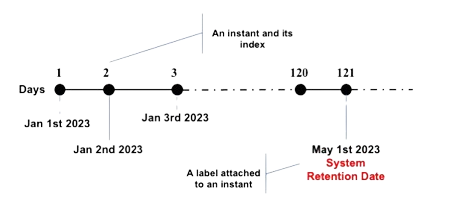
\includegraphics[width=\linewidth]{Clockpic.png}
   %   \caption{Example of Date Clock}
   %   \label{fig:dateclock}
 % \end{figure}
 %  \vspace{-2mm}
  %The data clock shown in Figure [\ref{fig:dateclock}] is a discrete-time clock. It is an example clock to represent the days starting from 1st of January of 2023. In this example, our labels are dates, with an additional text for eg., 121st instant is labeled with date and additional text $ \textit{retention date}$ representing a specific text to the label, which will be further used to check if statement execution is valid for a given retention time. %(which will be explained shortly).
  % Note that instants are strictly ordered, but the interval between two consecutive instants is futile in this logical model. 
%\end{example}

 \paragraph{Events}
An event is a flexible low-level synchronization primitive within the calculus that is used to construct a form of communication. The occurrence of an event might trigger processes. We specify a special time tick event $ e_{\#T}$, which will triggered after a period of specified simulation time $ T$. This $ T$ can be a bus cycle, processor cycle, or a real-world clock that generates events within the system's clock. In our date clock $ G_{d} =  \langle \mathcal{T}_{{d}},\  \prec_{{d}}, \ \mathcal{L}_{{d}}, \ \Lambda_{{d}},\  t_{{d}}  \rangle $ when the time unit $ t_d $ is a tick event $ e_{\#T}$ then the time advances in the clock for a next date. We explain more on time advance semantics later using figure \ref{fig:semP3}.
%Due to a lack of expressiveness in the privacy languages, we designed a privacy-aware policy language capturing the data protection requirements at various granularity's. Through this, we can provide exceptions in our policies involving different actors within distributed systems. Please refer to the paper for a more formal introduction and details on the language. This paper uses the same policy language to capture consent specifications. First, we need to define the entities-to-purposes, and purposes-to-action associations, where our actions specify entities for respective purposes that can perform what actions within a system. As mentioned each entity within the system is assigned an entity channel, $ P $ be the set of purpose names. In our settings, since our policy entry $ PE $  is a tuple with three attributes $ ( E, A, P)$ the consent specifications are a pair or two finitary relations where typically relations describe the possible connection between the elements of n-tuple. Hence, $ (\mathcal{P} : \mathcal{A}) $ consists of relation $ \mathcal{P}$ which assigns the entities to purposes, whereas the relation $ \mathcal{A}$ assigns the purposes to actions. which can be defined as follows:
%\[ \mathcal{P} \subseteq \ (\mathcal{E} \times P)  \quad \mathcal{A} \subseteq  \ ( A \times P) \]where,  $ A = \{ \textit{Use}, \textit{Collect}, \textit{Store}, \textit{Transfer}, \textit{Delete} \}$ represents a set of actions that can be performed on the data representing the whole data life-cycle and $ \mathcal{E}$ defines the entity channels in our calculus. We want to mention that actions are capabilities of sending, receiving, and performing GDPR-based operations on data over entity channels. The relation $ \mathcal{P}$ maps each entity channel with a purpose and relation $ \mathcal{A}$ maps the actions that could be performed for the purposes mapped.  We use the following notations for our consent specifications, $ \mathcal{P}(\epsilon)$ denotes the set of purposes attached to the entities. Here the domain of the  $ \mathcal{P}(\epsilon)$ relation is entities where the range is the purposes and we follow a similar analogy for the relation $ \mathcal{A}(\epsilon)$ which denotes the actions mapped with the purposes.
%we allow two more operations on consent mapping since the actions are dynamically assigned, if $ \exists A \ \ 
% s.t \ \ A \not \in dom(\mathcal{A})  $  then construct $ (\mathcal{P} : \mathcal{A})  \cup (A, P) %$  adds new actions to the purpose pair. similarly if  if $ \exists A \ \ 
% s.t \ \ A \in dom(\mathcal{A})  $ and if we want to remove the mapping then construct $ (\mathcal{P} : \mathcal{A})  \ set minus (A, P) $ removes the mapping from the respective purpose. We currently keep the entities and purposes fixed in the system mapping and actions are dynamically allocated at run-time.  


  

\section{Operational Semantics}
We want to bring the discussion to the operational semantics of our calculus stating 
that statically we do not have all the information within our system known,  since our system is based on a consent specification paradigm  and is interacting, open, and dynamically granted by the user at runtime. Even though knowing the system through static methods is interesting from a theoretical point of view, it may not be usable in a dynamic consent environment in practice. In this section, we introduce the operational semantics of the system via labeled transition rules which allows us to highlight the interactions with the environment.
In addition, the LTS provides operational semantics for any minimal system that can implement the GDPR specifications based on our consent specification during runtime. 
The standard way to represent the interactions within a system is by labeling the system's evolution. Hence we define a labeled transition system $ S \xrightarrow{\mu} S^{'}$, where system $S$ will execute the action indicated by label $ \mu $ and evolve to system $S^{'}$,
letting %and we use 
$ \mu$ %to 
range over the labels. The operational semantics come with enriched consent specification and run-time checks to avoid %the 
illegal handling of personal data. 
%The labeled transition system semantics of the calculus is the smallest set of transitions closed under the rules given in figure \ref{fig:semP1}. 
The labels that can be passed to perform actions are extended with that of standard $ \pi$  calculus. We distinguish four kinds of labels: standard communication labels, user interaction labels, and database interaction labels and time events.\\
$ \mu :: =  \gamma  \ | \ e_{\#T}  \ | \ a^e !(r) \ | \ a? (r) \ | \ a\leftarrow addCon(\rho) \ |  $
 $ \ \ \ \ \  \ \ a\leftarrow rmvCon( \rho) \ | \ a \leftarrow addRet(v) \ | \ a\leftarrow updRet( v) |  $
$ \  k \leftarrow store (\alpha) \ |  \  k \leftarrow delete (t) \  | \  k \  \leftarrow getdata (t)  $

The label $ \mu$ represents the internal actions of the system. Standard communication labels  $ a? (r)$ and $ a^e !(r) $ show the actions of sending/receiving term r onto/from the channel $ a$. The user interaction labels are as follows, $ a\leftarrow addCon(\rho) $ defines the action of sending a policy $ \rho $ onto the channel $ a $ to add consent, and label $ a\leftarrow rmvCon( \rho)$ shows the action of removing consent by sending the policy $ \rho $ on channel  $ a $  \\
At the center of the transition rules is the reduction relation $ \rightarrow$ on extended processes, mentioned in section \ref{}, which models the steps of computation.  
\cp{add reduction rules here }
 Since the database is the one giving access to store, delete, and access of personal data, we have three database interaction  labels $ k \leftarrow store (\alpha)  \ $ , $  k \leftarrow delete (t) $ and  $ \  k \  \leftarrow getdata (t) $. %labels $ k \leftarrow store (\alpha)  \ $, which is sending the personal data to our consent database via database channel $ k $; and action label  $  k \leftarrow delete (\alpha) $  sends the data $ \alpha $  to be deleted from the database via database channel $ k$; and to retrieve the data from the database we have the label $ \  k \  \leftarrow getdata (t) $ where the datastore sends the tags $ t $ data on the channel $ k $ which has a dual action from the database where $ k \  \rightarrow getdata (v)$ receives  personal data via the database channel. \\ 

 
\subsection{Auxiliary functions}
In our calculus, we introduce several auxiliary functions that support our operational semantics and are mainly used for privacy-related checks. %Since our runtime tags are set of users and purposes, 
We use the following functions to extract users and purposes from the tags.  Functions $ users(t)$ extract the users and $purpose(t)$ purposes, respectively.
$$
\begin{array}{ll@{\hspace{80pt}}ll@{\hspace{30pt}}l}
 users(t) =\{u \ | \ t= \pritag \land  u \in\manyset{u} %\land \manyset{u} \not = \emptyset 
 \ \} \\
  purpose(t) =\{p \ | \ t= \pritag \land  p \in\manyset{p} %\land \manyset{p} \not = \emptyset \land \manyset{u} \not = \emptyset 
  \}
 \end{array}$$
Let function $ \act(\cons, e, u,\manyset{p}) $ return a set of allowed actions for entity $ e$, user $ u$, purposes $ \manyset p $ in consent specification $ \cons $. 
  \[  \act(\cons,e, u,\manyset{p}) = \{ a \ | \ \cons(u) = \langle \Theta,\mathcal{R} \rangle\ \wedge\ 
 \exists
 p \in\manyset{p}\quad (e,p)\in \Theta(a) \} \]
We define a function $ \at(\cons,\eta, t) $ that, for any given tags and entity, extracts the allowed actions granted by the users in the consent $ \cons $. If the tags $t$ are empty, it implies that the data in question is non-private and all actions, i.e., use, collect, transfer, store, are granted. 
 \begin{equation*}
 \at(\cons,e, t) =
  \begin{cases}
   \bigcap \limits_{i=1}^{n} {\act%_i
    (\cons , e, u_i, \manyset{p} )},  \text{if} \  t = \langle \manyset{u},\manyset{p} 
\rangle \land \manyset{p} \not = \emptyset  \\% \land \manyset{u} = u_1 \dots u_n   \\
\{ \textit{use}, \textit{collect}, \textit{trans}, \textit{store} \},  \text{if}\ t = \emptyset \\
   {\mathit{\emptyset}},  \ \  \text{otherwise}
  \end{cases}
 \end{equation*}
 We have functions exclusive to database operations. Note that our database requests can be imagined in the form of queries, and we do not define the database process further to show the encoding but give an abstract idea data operation within the database. 
 Let $ datamap(u, w, \db)$ be the function that maps an entry to the database for a user. Since our database is a mapping of users and their respective values associated, a new private value $ w$ with its tags is added to the set of values $ v_t$. 
 %Note that the values can be private or non-private. 
%\begin{equation*}
 % datamap(u,w, \db) =
 % u \to \{ \manyset v_t \cup w \} \  \text{if}\ \db(u) = \manyset v_t \land w = v_t'\\
  % {\mathit{\emptyset}},  \ \ \quad    \text{otherwise}
% \end{equation*}
 \vspace{-1mm}
 \[ datamap(u,w, \db) = u \to \{ \manyset v_t \cup w \} \  \text{s.t}\ \db(u) = \manyset v_t \land w = v_t'\]
 \[ adddata(\manyset u,w, \db) =
    \ \bigcup \limits_{i=1}^{n} {\ datamap(u_i,w, \db)}, \ \text{s.t}  \ \manyset{u} = u_1 \dots  u_n \\ \]
we define function $ adddata(\manyset u , w, \db )$  which adds the mapping for all the users $ \manyset u$ with same data value. 
 %\begin{example}
    % consider the following example of the $ adddata$ function, where alice and bob wants common data $ jointaccountID$ needs to added for their individual mapping in database $ DB$. \\
     %$$ \begin{array}{ll@{\hspace{80pt}}ll@{\hspace{30pt}}l}
        % adddata( \{ \ alice, bob \ \}, JointaccountID, DB) = \\ 
         %\bigcup \limits_{i=1}^{2} {\ datamap(u_i,JointaccountID, DB)}, \ s.t  \ \manyset{u} = \{ alice, bob \}\\
    %\end{array}$$ 
 %\end{example}
\begin{figure*}[h!]
\centering
\boxed{
$$\begin{array}{c}

\ncondrule{L-Inp}{ \alpha = v_{t} \ \  \manyset u = \usr(t) \ \ \ \manyset p = \purp(t)  \\ \{use, collect \} \subseteq \at(e, \manyset u, \manyset p , \mathcal{C})
  \quad  G_d(i_{c}) \leq ret(  \manyset u, \mathcal{C})   }{ (G_d ,  \langle  \mathcal{C} ,   \mathcal{D} \rangle )\triangleright \ e[\![  a?(x ) \  .P ]\!] \  \ \toL{ a?( w )  } \ (G_d ,   \langle   \mathcal{C} , \mathcal{D}\rangle \ ) \triangleright \ e [\![ P \{ w  / x \} ]\!]} 
\qquad
\ncondrule{L-out}{  \  \manyset u = \usr(t) \ \ \ \manyset p = \purp(t) \quad \{use, transfer \} \subseteq \at(e, \manyset u, \manyset p , \mathcal{C})
 \\  \{use, collect \} \subseteq \at(f, \manyset u, \manyset p , \mathcal{C}) \quad \quad G_d(i_{c}) \leq ret(  \manyset u, \mathcal{C})   }{ (G_d ,  \langle  \mathcal{C} ,   \mathcal{D} \rangle) \triangleright \ e[\![ a^f!( v_{t}) .P ]\!] \   [5pt] \ \toL{ a^f!( v_{t})  } \  (G_d ,  \langle   \mathcal{C} , \mathcal{D} \rangle\ )\triangleright \ e [\![ P ]\!]} 
\qquad
\\[25pt] 
\ncondrule{L-comm}{  (G_d ,  \langle  \mathcal{C} ,   \mathcal{D} \rangle )\triangleright \ E \  \ \toL{ a?( w )  } \ (G_d ,  \langle  \mathcal{C} ,   \mathcal{D} \rangle ) \triangleright \ E' \quad (G_d ,  \langle  \mathcal{C} ,   \mathcal{D} \rangle ) \triangleright \ T \  \ \toL{ a^f!( w )  } \ (G_d ,  \langle  \mathcal{C} ,   \mathcal{D} \rangle ) \triangleright \ T' }{ (G_d ,  \langle  \mathcal{C} ,   \mathcal{D} \rangle ) \triangleright \  E \ || \ T \  \ \toL{ \tau  } \ (G_d ,  \langle  \mathcal{C} ,   \mathcal{D} \rangle ) \triangleright \  E' \ || \ T '} 
\qquad
\\[20pt] 
\ncondrule{L-Par}{  (G_d ,  \langle  \mathcal{C} ,   \mathcal{D} \rangle ) \triangleright \ E \  \ \toL{ \mu   } \ (G_d ,  \langle  \mathcal{C'} ,   \mathcal{D'} \rangle ) \triangleright \ E' \quad bc(\mu) \cap \ \textit{f}c(T) = \emptyset   }{ (G_d ,  \langle  \mathcal{C} ,   \mathcal{D} \rangle ) \triangleright \  E \ || \ T \  \ \toL{ \mu  } \ (G_d ,  \langle  \mathcal{C'} ,   \mathcal{D'} \rangle ) \triangleright \  E' \ || \ T } 
\qquad
\ncondrule{L-Res}{  (G_d ,  \langle  \mathcal{C} ,   \mathcal{D} \rangle ) \triangleright \ E \  \ \toL{ \mu  } \ (G_d ,  \langle  \mathcal{C} ,   \mathcal{D} \rangle ) \triangleright \ E' \ \quad a^e \not \in \  Fc(\mu) }{ (G_d ,  \langle  \mathcal{C} ,   \mathcal{D} \rangle ) \triangleright \  (\nu a^e )E \ \  \ \toL{ \mu  } \ \langle   \mathcal{C} , \mathcal{D} \rangle\ \triangleright \ (\nu a^e )  E' \ } 
\qquad
%\\[27pt] 
%\ncondrule{L-Tau}{  (G_d ,  \langle  \mathcal{C} ,   \mathcal{D} \rangle )\triangleright \ E \  \ \toL{ \mu_1  } \ (G_d ,  \langle  \mathcal{C} ,   \mathcal{D} \rangle ) \triangleright \ E' \quad (G_d ,  \langle  \mathcal{C} ,   \mathcal{D} \rangle ) \triangleright \ T \  \ \toL{ \mu_2  } \ (G_d ,  \langle  \mathcal{C} ,   \mathcal{D} \rangle ) \triangleright \ T' }{ (G_d ,  \langle  \mathcal{C} ,   \mathcal{D} \rangle ) \triangleright \  E \ || \ T \  \ \toL{ \tau  } \ (G_d ,  \langle  \mathcal{C} ,   \mathcal{D} \rangle ) \triangleright \  E' \ || \ T '} 
%\qquad
\\[20pt] 
\ncondrule{L-Repl}{  (G_d ,  \langle  \mathcal{C} ,   \mathcal{D} \rangle ) \triangleright \ e[\![ \ P \ | \ *P \ ]\!]  \  \ \toL{ \mu  } (G_d ,  \langle  \mathcal{C'} ,   \mathcal{D'} \rangle ) \ \triangleright \ E \quad  }{ (G_d ,  \langle  \mathcal{C} ,   \mathcal{D} \rangle ) \triangleright \ e[\![  \ *P \ ]\!] \ \toL{ \mu  } \ (G_d ,  \langle  \mathcal{C'} ,   \mathcal{D'} \rangle )\triangleright \ E } 
\qquad
\ncondrule{L-split}{  (G_d ,  \langle  \mathcal{C} ,   \mathcal{D} \rangle ) \triangleright \ e[\![ \ P  \ ]\!] \ || \ e[\![ \ Q \  ]\!] \  \ \toL{ \mu  } \ (G_d ,  \langle  \mathcal{C'} ,   \mathcal{D'} \rangle ) \triangleright \ E \  }{ (G_d ,  \langle  \mathcal{C} ,   \mathcal{D} \rangle ) \triangleright \  e[\![ \ P \  | \ Q   \ ]\!]  \ \  \ \toL{ \mu  } \ (G_d ,  \langle  \mathcal{C'} ,   \mathcal{D'} \rangle ) \triangleright \ E \ } 
\qquad
\\[27pt]
\end{array} $$}
\caption{\label{fig:semP1} 
 Standard execution rules in
CCAL}
\end{figure*} 
\begin{figure*}[h!]
\centering
\boxed{
$$\begin{array}{c}
 \ncondrule{L-Storedata}{ \alpha = v_{t} \ \  \manyset u = \usr(t) \ \ \ \manyset p = \purp(t) 
 \{use, store \} \subseteq \at(e, \manyset u, \manyset p , \mathcal{C})
 \quad \\  \mathcal{D}' = adddata(\manyset u , w , \mathcal{D}) \quad G_d(i_{c}) \leq ret( \manyset u, \mathcal{C})  }{ (G_d , \langle  \mathcal{C} ,   \mathcal{D} \rangle) \triangleright \ e[\![ k \leftarrow store(\alpha).P ]\!] \ \\ [5pt] \toL{ k ? \leftarrow store(w)  } \ \\   (G_d , \langle   \mathcal{C} , \mathcal{D}' \rangle \ ) \triangleright \ e [\![ P \{ w  / \alpha \} ]\!]} 
\quad \quad \quad
\ncondrule{L-Deldata}{ \alpha = v_{t} \ \  \manyset u = \usr(t) \ \ \ \manyset p = \purp(t) 
\{use, delete \} \subseteq \at(e, \manyset u, \manyset p , \mathcal{C})
 \quad \\ \mathcal{D}' = deldata(\manyset u , w, \mathcal{D} ) \quad G_d(i_{c}) \leq ret( \manyset u, \mathcal{C}) }{(Gclk ,   \langle  \mathcal{C} ,   \mathcal{D} \rangle) \triangleright \ e[\![k \leftarrow delete(\alpha).P ]\!] \  \\ [5pt]  \ \toL{ k ? \leftarrow delete(w) } \ \\ (Gclk ,  \langle   \mathcal{C} , \mathcal{D}' \rangle\ ) \triangleright \ e [\![ P \{ w  / \alpha \} ]\!]} 
\qquad
\\[32pt] 
 \ncondrule{Lin-Getdata}{ t = \langle \manyset u , \manyset p \rangle \ \ 
 \{use, collect \} \subseteq \at(e, u, \manyset p , \mathcal{C})
 \quad  \delta = getdata( u , \manyset p , e , \mathcal{C} ) \quad  \\ G_d(i_{c}) \leq ret(  u, \mathcal{C})  }{ (G_d , \langle  \mathcal{C} ,   \mathcal{D} \rangle) \triangleright \ e[\![ k \leftarrow getdata(t).P ]\!] \   \\ [5pt] \toL{ k  \leftarrow getdata(w)  } \ \\   (G_d , \langle   \mathcal{C} , \mathcal{D} \rangle \ ) \triangleright \ e [\![ P \{ w  / \alpha \} ]\!]} 
\quad \quad \quad
 \ncondrule{Lout-Getdata}{ \alpha = v_t  \ 
 \{use, collect \} \subseteq \at(e, u, \manyset p , \mathcal{C})
 \quad  t = \langle u , \manyset p \rangle \ \\ \quad G_d(i_{c}) \leq ret(  u, \mathcal{C})  }{ (G_d , \langle  \mathcal{C} ,   \mathcal{D} \rangle) \triangleright \ e[\![ k \rightarrow getdata(\alpha).P ]\!] \  \\ [5pt] \toL{ k  \rightarrow getdata(w)  } \ \\   (G_d , \langle   \mathcal{C} , \mathcal{D} \rangle \ ) \triangleright \ e [\![ P  ]\!]} 
\qquad
%\nrule{Lo
\\[27pt]
\end{array} $$}
\caption{\label{fig:semP4} 
 Execution rules for  database query statements in
 PAOL.}
\end{figure*} 



we define functions $delmap(u, \db) $ and $ deldata(\manyset u, \db)$ to delete the mapping of the users from the database.  This works analogously to adding the data mappings. 
  \[ delmap(u, \db) =  u \to \emptyset \ s.t \ \exists u \land \db(u) = \manyset v_t  \]
    $ deldata(\manyset u, \db) =
    \ \bigcup \limits_{i=1}^{n} {\ delmap(u_i, \db)}, s.t  \ \manyset{u} = u_1 \dots  u_n \\ $
 We also have function $ret(\manyset{u}, \cons) $ to extract the retention of the users $ \manyset{u} $ from their respective consent.
      
The rules defining the LTS transitions $ S \xrightarrow{\mu} S^{'}$, are given in four separate parts, first we give standard transition rules in figure \ref{fig:semP1}, the database interaction rules in \ref{fig:semP4}, the user interaction rules in figure \ref{fig:semP2}, and global time transition rules in figure \ref{fig:semP3}. The overall structure is similar to the standard $ \pi $ calculus with our privacy extensions. According to rule $\scriptsize \text{ [L-INP]}$, the input prefix $ a?(x)$ may interact with the input action $ a?(w)$, the rules apply for both personal and non-personal data rule $\scriptsize \text{ [L-INP]}$ denotes the process of sending data on the channel $ a $, since the data comes with runtime tags in our semantics, using $ tags(v_{t}) $ function tags of the data is extracted and respectively the users and purposes attached with the tag. Premises mainly check if the bounded entity $ e $  listening on the channel  $ a$ has access  $ \textit{use} $ and $ \textit{collect}$ in order to receive the value over the channel and perform active substitution of data within the local scope. Action credentials are checked for tags received against the users consent. %For the users $ u$ and purposes $ p$ and this is checked against the global consent $ \cons $ given by the users. 

Retention is checked if the current instant of the Global clock $G_d(i_c)$ is less than or equal to the retention in the consent for all users $ \manyset{u}$. If the access is not available or the retention date is invalid in the consent, the rule gets blocked and does not proceed further. % If all premises hold the prefix is satisfied and then continue as process P.
Note that if the data has empty tags attached, indicating it's public data, the communication proceeds with privacy checks being true, and all the premises hold. Rule $ \scriptsize \text{[L-OUT]}$ the output prefixed $a^f!(v_t) $ process may react with the output action $ a^f!(v_t)$ and continue as process P if all the privacy checks are satisfied. To send privacy value $ v_t$ over the channel, we have to specify the entity location where communication has to happen $ a^f$. Action credentials i.e, $ \textit{use}, \textit{transfer}$ are checked for the tags attached, current entity $ e$ against the consent $ \cons$ and retention is checked  w.r.t global clock and since we are transferring the data to entity $ f$ we check if the entity is able to $ \textit{use}, \textit{ collect}$ the data in the consent. Communication arises in rule $ \scriptsize \text{[L-COMM]}$ by means of a $ \tau $ action obtained by a synchronisation of an $ a?(w)$ action with a $ a^f!(w)$ action. Rule $ \scriptsize \text{[L-RES]}$ states that actions are closed under the restriction operation provided that the restricted name does not occur freely in any action. Note that a restriction of a channel does not inhibit the use or mentioning of other names.  Rule $\scriptsize  \text{[L-PAR]} $ states that the actions are closed under the parallel composition provided that there is no name conflict between the bounded names of the actions and the free names of the parallel composition.  Rules $ \scriptsize \text{[L-SPLIT]}$ $ \scriptsize \text{[L-REPL]}$ are standard rules that assume alpha conversion. \\
Figure \ref{fig:semP4} shows the database interaction rules, rule $ \scriptsize  \text{[L-STOREDATA]}$ with database process expression prefix observes the label $ k \leftarrow store(w) $, checks for action credentials, validity of retention and as a result stores the data in database, if the same data with multiple users is received data is stored for all the users individually. Rule  $ \scriptsize  \text{[L-DELDATA]}$ shows the process interacting with  $ k \leftarrow delete(w) $ label performs privacy checks and deletes the data from the respective users. whereas rule $ \scriptsize  \text{[L-GETDATA]}$ shows a process inetraction with label $ k \leftarrow getdata(w) $ gets the runtime tags attached with users and purposes, upon satisfying privacy checks process will have a dual  \cp{check getdata rule}
\begin{figure*}[h!]
\centering
\boxed{
$$\begin{array}{rcl}
 \ncondrule{L-AddPol}{ (u) == (v) \ \quad  \Theta' =  InsertPol(\Theta, \rho ) }{ \quad \quad  (G_d ,\langle (u \to \langle \Theta , \mathcal{R} \rangle );  \mathcal{C} , \mathcal{D} \rangle) \triangleright \ v[\![ x \leftarrow addCon(\rho).P ]\!] \\ [5pt]  \quad  \ \toL{ x \leftarrow addCon( w ) } \\   (G_d ,\langle (u \to \langle \Theta' , \mathcal{R} \rangle );  \mathcal{C} , \mathcal{D}) \rangle) \triangleright \ e [\![ P \{ w  / \rho \} ]\!]} 
\qquad
\ncondrule{L-RemPol}{ (u) == (v) \ \quad \Theta' =  RemPol(\Theta, \rho ) }{ (G_d ,\langle (u \to \langle \Theta , \mathcal{R} \rangle );  \mathcal{C} , \mathcal{D} \rangle) \triangleright \ v[\![ x\leftarrow  remCon(\rho).P ]\!] \\ [7pt]  \quad  \ \toL{ x\leftarrow remCon( w )  } \\ \   (G_d ,\langle (u \to \langle \Theta' , \mathcal{R} \rangle );  \mathcal{C} , \mathcal{D} \rangle) \triangleright \ e [\![ P \{ w  / \rho \} ]\!]} 
\qquad
\\[32pt]
 \ncondrule{L-AddRet}{ (u) == (v) \ \quad  \mathcal{R'} = w }{ (G_d ,\langle (u \to \langle \Theta , \emptyset \rangle );  \mathcal{C} , \mathcal{D} \rangle) \triangleright \ v[\![ x \leftarrow  addRet(r).P ]\!] \  \\ [7pt]  \quad \toL{ x \leftarrow addRet( w ) } \\ (G_d ,\langle (u \to \langle \Theta , \mathcal{R'} \rangle );  \mathcal{C} , \mathcal{D}) \rangle) \triangleright \ e [\![ P \{ w  / r \} ]\!]} 
\qquad
 \ncondrule{L-UpdRet}{ (u) == (v) \ \quad  \mathcal{R}' = w }{ (G_d ,\langle (u \to \langle \Theta , \mathcal{R} \rangle );  \mathcal{C} , \mathcal{D} \rangle) \triangleright \ v[\![ x \leftarrow  updRet(r).P ]\!] \  \\ [7pt]  \quad \toL{ x \leftarrow updRet( w ) } \\ (G_d ,\langle (u \to \langle \Theta , \mathcal{R'} \rangle );  \mathcal{C} , \mathcal{D}) \rangle) \triangleright \ e [\![ P \{ w  / r \} ]\!]} 
\qquad
\\[37pt]
\end{array} $$}
\caption{\label{fig:semP2}  
 Execution rules for user-interaction statements in
 PAOL.}
\end{figure*}



\begin{figure*}[t]
\centering 
\boxed{
$$\begin{array}{rcl}
 \ncondrule{L-ClockTick}{ \ \ t_{{d}} = e_{\#T} \ \ \  \mathcal{U}= alluser(\db) \ \  RetOk ( \mathcal{U}, \db, G_d(i_c)) }{   (\langle \mathcal{T}_{{d}},  \prec_{{d}},  \mathcal{L}_{{d}},  \Lambda_{{d}},  t_{{d}}  \rangle , \langle \cons , \db \rangle) \triangleright E  \ \\ \toL{ e_{\#T} }   \\  (\langle \mathcal{T}_{{d}}',  \prec_{{d}},  \mathcal{L}_{{d}}',  \Lambda_{{d}}',  t_{{d}}  \rangle , \langle \cons , \db \rangle) \triangleright  E } 
\quad
\ncondrule{L-ClockTick delete}{ \\ t_{{d}} = e_{\#T} \  \mathcal{U}= alluser(\db) \  \neg RetOk ( \mathcal{U}, \db, G_d(i_c)) ) \  \db' = DelExpired(\mathcal{U})  }{  \quad  (\langle \mathcal{T}_{{d}}, \prec_{{d}}, \mathcal{L}_{{d}},  \Lambda_{{d}}, t_{{d}}  \rangle , \langle \cons , \db \rangle) \triangleright  E   \\  \ \toL{ e_{\#T} }  \\  (\langle \mathcal{T}_{{d}}',  \prec_{{d}},  \mathcal{L}_{{d}}', \Lambda_{{d}}',\  t_{{d}}  \rangle , \langle \cons , \db' \rangle) \triangleright  E } 
\quad
\end{array} $$}
\caption{ \label{fig:semP3} 
 Execution rules for user-interaction statements in
 PAOL.}
\end{figure*}

Figure \ref{fig:semP2} shows user interaction rules, users in our system are program elements and are statically available. Rule $\scriptsize \text{[L-ADDPOL]}$ defines a process where user adds consent via prefix $ x \leftarrow addCon(\rho)$ where the users identity is validated and sends the policy $ \rho$ via channel $ x$ after the process interacts with the label, the policy is added to the consent specification. Note that here, the respective user from the session is matched against the user identifier in the consent specification.
 The rule $ \scriptsize \text{[L-REMPOL]}$ removes the policy bindings from the consent specification respectively.
 The rules $\scriptsize  \text{ [L-ADDRET]}$ and $ \scriptsize  \text{[L-UPDRET]}$ add and update the retention in the consent specification within the respective user session. 
 

 Figure \ref{fig:semP3} defines two rules specifying the global clock semantics.
 Semantics for the time model does not explicit the computation time of each operation. In particular, two instants of global date clock $ G_d$ are independent of computation time in between.  When the time unit $ t_d$ has a tick event, the system interacts with a time event label $ e_{\#T}$  the rule $  \scriptsize  \text{ [L-clocktick]}$ advances the clock by adding new instant $ \mathcal{T}'_d$, label $ \mathcal{L}'_d$ and new mapping $ \Lambda'_{d} $. For each clock advancement, the retention date of all the users in the database is checked against the system clock, if the retetion check does not satisafy we have rule rule $  \scriptsize  \text{[L-Clocktick delete]}$ which deletes of user data with expired retention dates, meaning if the retention of any users within the database is greater than the current instant of the global clock, then such user's data will be deleted from the database.  %we abstract the deletion away via a database operation $ \scriptsize  DelExpired(\mathcal{U})$.
 %denotes a process that sends non-private data on a channel, if the data structure is not of the form $ \langle x, y\rangle$ where $x = id $ and $y = \tau$ we consider it as non-sensitive data input/output communications. we do not check for any private properties on such data. These are considered non-harmful communications as it does not involve any personal data. Rule $ [L-PIN]$ denotes the process of sending private data of the form $ \langle x, y\rangle$  tagged with purposes at runtime denoting $ \langle x, y\rangle_{z}$ on channel $ a $ action checks the premise if the data has  $x = id $, $y = \tau$ and from the $\textit{purp}$ function if the tagged purposes belong in the domain of $ \mathcal{P}(e)$ and the data is received only if the action $ \{ collect\}$ belong in the domain of $ \mathcal{A}(e)$ from our consent mapping. In our interpretation collection of data is interpreted as receiving of private data, if the entity $ e$ has right actions i.,e $ \{ collect \}$ for right purposes belonging to $ \mathcal{P}(e)$ as specified in consent specification then the data is allowed to be collected or received. \\

%Rule $ [L-OUT] $ denotes an action of sending private data. Premise checks if the consent mapping for the actions $ \mathcal{A}(e) $ consists of $ \{transfer\} $. We interpret the private data sending as action $ \textit{transfer} $ in the privacy paradigm. Here note that the output actions also specify the entities where the transfer should take place as well.  Rule $ [L-DBIN]$  denotes an action of sending private data to the database store through channel $ k$ that is allowed to store the personal data if the  entity is mapped to $ \mathcal{A}(e) $ consists of actions  $ \{collect, store\} $ Similarly, Rule $ [L-DBOUT]$ checks if the stored private data in the database can be used which are checked in premise if the  $ \mathcal{A}(e) $ consists of actions  $ \{collect, store, use\} $  use action denotes the data can be used by the entity via the database. Rule $ [L-ADDCONS]$ adds the additional consent to our consent mapping since our entities and purposes are fixed within the system modeling the only dynamically allocated resource is actions associated with the entities and purposes. Hence adding consent if adding additional actions, the premise checks, if the value sent, does not belong in the domain of actions $ \mathcal{A}(e)$ then as we saw in the earlier section we add the additional consent $ (\mathcal{P}: \mathcal{A } )\ \cup (a,p) )$ symmetric to this rule $ [L-ADDCONS]$ does the symmetric action where if the action belongs in the $ \mathcal{A}(e)$ then label $  a?rmv(a, p)$ removes the action value passed from the specification i.,e $ (\mathcal{P}: \mathcal{A }) \ \cap (a,p) $. Rule $ [L-COMM], [L-PAR],[L-RES],[L-REP],$ are standard $ \pi$ calculus rules for communication, parallel communication, restriction, and replication which are symmetric to reduction rules. 


\subsection{Thoughts on Error Handling when lacking consent }
The semantics of the calculus does not include runtime error handling. If a runtime error occurs in one of the processes, the execution of the process will stop, and the process thread will get stuck. Since our calculus is mainly concerned with consent-based processing of user data, errors might occur at runtime due to a lack of consent for handling personal data. One alternative to overcome such errors is the use of a \emph{dynamic consent interaction dialogue with the user}, where a dialogue box is introduced asking for the required consent from the user. Regarding GDPR, this could be reflected by opt-in/opt-out requests, that user allow dynamically at runtime, we can further refine the options to:
1) \emph{Allow-once:} for temporary consent, with a new dialogue next time when consent is needed. 
2) \emph{Allow-Always:} for changing the consent so that it is used for further processing. 
Failure to apply any rule within the LTS will result in runtime errors that can be modeled within our calculus. The process in the syntax can be extended with three different errors: standard errors, access errors, and retention errors. 
\vspace{-1mm}
     \[ P ::=    \ \text{Err}  \ | \ \text{accesErr}   \ | \ \text{retErr}  \]  
We give error semantics example for two LTS rules for input message in fig \ref{fig:errsem}. However, the rest of the rules are straightforward and can be written in a similar style. To explain error semantics, we consider the $ \scriptsize  \text{[L-InpAccessErr]}$ rule, listening on a  channel upon receiving personal data premises checks for credentials for right access i.e., use collect and lack of access in current consent results in runtime access error. Similarly, if the global clock has exceeded user retention, results in a retention error given in the rule  $ \scriptsize  \text{[L-InpRetErr]}$.

\begin{center}
\begin{figure*}[h]
\centering
\boxed{
$$\begin{array}{c}

\ncondrule{L-InpAccessErr}{ \alpha = v_{t} \ \  \manyset u = \usr(t) \ \ \ \manyset p = \purp(t)  \\ \neg (\{use, collect \} \subseteq \at(e, \manyset u, \manyset p , \mathcal{C}))
  \quad  G_d(i_{c}) \leq ret(  \manyset u, \mathcal{C})   }{ (G_d ,  \langle  \mathcal{C} ,   \mathcal{D} \rangle )\triangleright \ e[\![  a?(x ) \  .P ]\!] \  \ \toL{ a?( w )  } \ (G_d ,   \langle   \mathcal{C} , \mathcal{D}\rangle \ ) \triangleright \ e [\![ \text{accessErr} ]\!]} 
\quad
\ncondrule{L-InpRetErr}{ \alpha = v_{t} \ \  \manyset u = \usr(t) \ \ \ \manyset p = \purp(t)  \\ \{use, collect \} \subseteq \at(e, \manyset u, \manyset p , \mathcal{C})
  \quad  \neg (G_d(i_{c}) \leq ret(  \manyset u, \mathcal{C}))   }{ (G_d ,  \langle  \mathcal{C} ,   \mathcal{D} \rangle )\triangleright \ e[\![  a?(x ) \  .P ]\!] \  \ \toL{ a?( w )  } \ (G_d ,   \langle   \mathcal{C} , \mathcal{D}\rangle \ ) \triangleright \ e [\![ \text{RetErr} ]\!]} 
\qquad
\\[29pt]
\end{array} $$}
\caption{\label{fig:errsem} 
 Error Execution rules for Input statement}
\end{figure*} 
\end{center}


\vspace{-5mm}
\subsection{Reflection on semantics by example: E-Health System}
\label{sec:casestudy}
Nowadays, many user-centric services are delivered through smart systems and internet-connected devices. It is crucial to model these pervasive systems within the healthcare sector, given the extensive and sensitive nature of information managed by E-health systems. This includes individual details like medical history, diagnostic reports, treatment plans, etc. E-health systems often employ sensors and monitors to effortlessly collect patient data, with continuous monitoring and extracting insights; while all of this makes the user interaction with the hospital system easier, it still fails to empower individuals privacy.
%Cloud systems are integrated into E-health systems to off-load services onto the cloud to increase scalability and performance. 
%Usually, these cloud partners are third-party services hidden from users' sight when using patients' personal data. Hence, 
We model an E-health system using CCAL, which mainly involves user's personal data flow within the systems by current consent among various entities.  Let %. Where 
$ \textit{Doctor}$, $ \textit{Nurse}$, $ \textit{Patient}$ and $ \textit{Lab}$ be the various system components. 
The workflow of the E-health scenario is as follows: 
    1) User Alice is registered in the system and can manage consent at any stage in processing.
    2) Alice provides her blood samples to a lab to generate some results.
    3) Lab collects the sample data, performs computation, saves reports in the storage system, and sends a copy of them to the Nurse.
    4) Nurse collects the lab reports, performs analysis, and sends them to the Doctor.
    5) Doctor retrieves patient details from the storage, receives an analysis report from the Nurse, and performs further diagnosis.\\
For this concrete scenario, we assume global date clock $ G_d$ in the current configuration is dated 31st March 2023 and $ \cons_h $ and $ \db_h$ as the global consent and database given as follows, \\
%
$\begin{array}{lcl}
 \textstyle  \cons_h &  \triangleq & (alice \rightarrow  \{   use \rightarrow \langle (doctor, trt) , (nurse, trt)\rangle  ,\\
 & &  collect \rightarrow \langle\{ (doctor, trt) , (nurse, trt)\rangle \} , \\
 & & store \rightarrow \langle\{ (doctor, trt) , (nurse, trt)\rangle \}  , \\ 
 & & trans \rightarrow \langle\{ (doctor, trt) , (nurse, trt)\rangle \} ,  \\
 & & \text{1st April 2023} )  \\
 \db_{h} &  \triangleq & (alice \rightarrow  \{ Id_{t1}, address_{t2}\} , bob \rightarrow \{ reports_{t3} \})  
\end{array}$
Here user Alice consent allows entities $ \textit{doctor}$ , $ \textit{nurse}$ to $ \textit{use}$, $ \textit{collect}$ data for purpose of $ \textit{trt}$. The database currently stores data values $ \textit{Id}$, $ \textit{Address}$ along with their private tags.
We model the system based on the specifications as follows,
$\begin{array}{lcl}
\textit{System } & \triangleq &  (G_d , \langle \cons_h, \db _h\rangle ) \triangleright  Doc\, | \, Nur \, | \,  Patient \, | \, Lab \\
\textit{Patient  } & \triangleq & alice \ [\![  a \leftarrow addCon(\rho_1).  a \leftarrow addRet(r) \\
&  &   b^{lab}!(sample \ \textbf{tag} \ {\{alice\}, \{trt,lab\}}) ]\!] \\
\text{Lab }&  \triangleq &  l  [\![  b?(x \ \textbf{tag} \ t ). \\
& &  c^{nur}!(rep \ \textbf{tag} \ {\{alice\}, \{trt,lab\}}) ]\!] \\
 \text{Nur } & \triangleq  & nur [\![  c?(y \ \textbf{tag} \ u ).  k \leftarrow store (y  \ \textbf{tag} \ u)\\
 & & d^{doc}!(analysis \ \textbf{tag} \  ({\{alice\}, \{trt,lab\}})) ]\!]  \\
 \text{Doc  } & \triangleq  & doc [\![  d?(z). k \leftarrow getdata((\{ alice\}, \{trt\})).  \\
 & &  k?(x) .  k \leftarrow delete(y  \ \textbf{tag} \ u) ]\!] \\
\end{array}$
Here doctor, nurse, and lab are entities in the system and the patient is the user. Patient alice updated her consent by sending her policy $ \rho_1$ and retention $r$ via channel $ a $. Here the user interaction rules $ \scriptsize \text{[L-ADDPOL]}$ and $ \scriptsize \text{ [L-ADDRET]}$ are applied respectively updating the global consent and sends her tagged personal data $ \text{sample}$ to the lab via channel $ b$. Lab $ l$ gets a sample $x \ \textbf{tag} \ t $ from a patient on channel $ b$, lab has both use and collect rights for trt purpose in the consent and retention checks holds hence rule $ \scriptsize \text{[L-Inp]}$, applies, after local computation process sends lab reports $rep \ \textbf{tag} \ {(\{alice\}, \{trt,lab\})}$ to nurse via channel $ c$ and respective actions, use and transfer and retention validity checks are done by $ \scriptsize \text{[L-out]} $. 
Nurse receives data from the lab via channel $ c$, privacy checks are done by rule $ \scriptsize \text{[L-out]} $, nurse stores the data to database via  rule $ \scriptsize \text{[L-STOREDATA]} $performs analysis and sends the analysis to the entity doctor via channel $ d$. Here again the respective rules checks for valid privacy requirements. The doctor receives an analysis from the Nurse and retrieves other data of the user from the database applying rule $ \scriptsize \text{[L-GETDATA]}$  however, when doctor tries to delete the data in database via database channel $k$ action use and delete are checked against the consent via rule $ \scriptsize \text{ [L-DELDATA]}$, and fails to apply the rule stopping the consent violation. With such a modeling example can help understand and reason about consent needed from the users to perform or analyse the data and provide services accordingly. The example also showcases when the data belongs to multiple users, how the rule checks for the consent from each  user. 




%Upon removal of consent, any attempts to access the personal data will fail in the rule application and the process enters an error state. 
%Here framework allows a patient to be an integral part of her personal data processing and any access to personal data is handled as per the available consent.
\vspace{-3mm}
\section{Implementation}
\label{sec:implem}
Maude is a powerful tool for implementing various semantics to experiment with quick prototypes for trying examples and proving properties. It is a high-level language and high-performance system supporting equational and rewriting logic computation. We use Maude as a metalanguage in which the syntax and semantics of the CCAL  can be formally defined. It is easier to scale the implementation based on the executable in Maude. We have formalized the operational semantics,  which provides a prototypic environment for our specification. We validate the running example from the case study with two versions, consented and unconsented specifications. The full executable in Maude and the running example can be downloaded from \url{https://github.com/Chinmayiprabhu/CCALexecutable.git}. 

\section{Related Work }
\label{sec:related}
Notions such as privacy by design (PbD)~\cite{CavoukianC09}, data protection by design and default~\cite{EUA2014}, and legal compliance appear quite often in the literature; despite much ongoing work in this direction, the research community agrees about the need of practical guidance on such notions~\cite{utz__2019, kutylowski_gdpr_2020 }. Schneider indicates that privacy principles, such as PbD, go through various levels of abstraction from their conceptual models during design time until software implementation and do not entirely guarantee privacy~\cite{schneider_is_2018}. Hence, there is a need for privacy-aware languages that help capture software design models with data privacy constructs that facilitate the check of privacy principles.
The purpose based processing data is vital to privacy and formal approaches such as 
privacy-aware role-based access control models consider purposes, roles, and obligations to specify the access control policies and role-based access control (RBAC) models enriched with purpose-awareness~\cite{yang_purpose-based_2007,byun_purpose_2005,masoumzadeh_purbac_2008 } for enterprise data handling have been previously well-explored; these authorization models fail to capture the current regulatory requirements and consider only organizational interests and not user preferences.
%
In existing language-based approaches, a programming language with privacy principles is checked either statically or at runtime. Researchers have previously explored information flow analysis to make  programs comply with  privacy policies, many of these
approaches use static techniques~\cite{TokasOR22, sen_bootstrapping_2014, myers_protecting_2000}, which will not be enough to fully capture %automate 
GDPR compliance, since elements, such as consent change at runtime. 
Some runtime checking work, as in~\cite{TokasO20, KaramiBJ22}, the former considers a subset of GDPR elements that we address and the latter has built in consent management operations but are not considering process calculi.
%
There are well-explored works using pi-calculus in the state-of-the-art reasoning security and privacy properties. $\pi$-calculus serves as both a modeling language for systems and a tool for validating various properties. For instance, applied pi calculus, as discussed in \cite{abadi2017applied}, facilitates the specification and automatic analysis of security protocols Type system have been employed with $ \pi$ calculus in number of papers to reason about access control and policy authorisations however the exploration of the GDPR concepts is not prevalent in these works.. Closest to our work is the Privacy Calculus which proposes a modelling language incorporating the notions like purpose, consent and privacy policies. Nevertheless, in contrast to our approach, Privacy Calculus relies on static techniques to model consent, since consent is dynamic given on the fly static approaches will not be enough to reason about compliance.  They also do not consider retention and deletion of data. In the direction of a general study of GDPR and legal compliance,
Ranise and Siswantoro~\cite{ranise_automated_2017} propose an approach for privacy-aware automated legal compliance checking by using tools for policy analysis on efficient SMT solvers. Unfortunately, this was proposed before GDPR and did not consider crucial elements like consent, actions, entities, and other GDPR requirements. Piras~{et al.}~\cite{piras_defend_2019} propose the design of an architecture abiding by GDPR requirements. However, this approach lacks implementation details on compliance and does not address data interoperability at lower system operations, unlike our approach, where enforcement of data subjects' preferences and monitoring inconsistency with consent is handled on a data level, guaranteeing a concrete notion of compliance.
%Further away from the techniques shown in this paper, there is a line of research that explores compliance checking through blockchain technology; Vargas~\cite{vargas_blockchain-based_nodate} proposes a blockchain-based automated tool for compliance that considers consent operations and the purpose of processing. Similarly, Truong~{et al.}~\cite{truong_gdpr-compliant_2020} propose a Blockchain-based personal data management compliance with the GDPR platform, guaranteeing GDPR requirements like transparency and accountability. However, blockchain's immutability, i.e, ledgers can never be erased, clashes with GDPR's "right to be forgotten", and even if personal data is stored off-chain, any record on the chain will result in violation of GDPR in the platform. \\
%Privacy by Design (PbD)~\cite{CavoukianC09} and data protection by design and default~\cite{EUA2014}, encourage a multidisciplinary approach to identify potential privacy risks and develop effective mitigation strategies. It promotes transparency, accountability, and user-centricity, ensuring that individuals' privacy rights are respected throughout the lifecycle of a product or service. 

%\emph{Formal Methods and privacy : }
\section{Conclusion }
\label{sec:conclusion}
This paper proposes a modeling language that integrates privacy features into core $\pi $ calculus and explores how syntax and semantics can be used to ensure personal data handling by design and default. The motivation behind incorporating privacy constructs, along with existing challenges in the field, is explored, emphasizing their integration into calculus for enforcing consent-based data processing. Operational semantics, offering such abstractions, are presented, and an evaluation is conducted through a healthcare example and a Maude-based simulation environment that allows us to simulate programs and experiment with our new calculus features. Our currently proposed semantics are fixed to a concrete interpretation of GDPR terminology. Exploring how to parametrize the transition rules concerning desired personal data handling checks according to different data privacy legislations and domain expertise would be interesting. The proposed data privacy checks introduce notable runtime overheads for every transition rule handling data, prompting future investigation into reducing checkpoints while still ensuring compliance. Techniques like behavioral types ~\cite{BehaviouralTypes2016} could be explored to statically approximate the required checks and offer a type system for the calculus. To demonstrate correctness, the paper aims to prove bisimulation equivalence for systems.

\bibliographystyle{abbrv}
 \bibliography{refs} 

\end{document}
